\documentclass[11pt]{article}
\usepackage[a4paper, margin=1in]{geometry}
\usepackage{graphicx}
\usepackage{hyperref}
\usepackage{caption}
\usepackage{subcaption}
\usepackage{amsmath}
\usepackage{multicol}
\usepackage{times}
\usepackage{authblk}
\usepackage{booktabs}
\usepackage{array}
\usepackage{xcolor}
\usepackage{float}
\usepackage{wrapfig}
\usepackage{siunitx}

% Enhanced formatting
\setlength{\parskip}{0.5em}
\setlength{\parindent}{0pt}
\hypersetup{
    colorlinks=true,
    linkcolor=blue,
    citecolor=blue,
    urlcolor=blue
}

% Custom colors
\definecolor{mauryanblue}{RGB}{30,144,255}
\definecolor{granitetext}{RGB}{64,64,64}

\title{\textbf{Echoes of Empire: A Comprehensive Study of the Barabar Caves and Surrounding Sites}}
\author[1]{Justin T. Bogner}
\affil[1]{Independent Researcher, Pelican's Perspective}
\date{August 2025}

\begin{document}
\maketitle

\begin{abstract}
This report presents an exhaustive, multidisciplinary analysis of the Barabar Caves complex in Bihar, India, and allied archaeological locales. Drawing upon recent field studies, high-precision 3D laser scans, acoustic testing, petrographic assays, and epigraphic surveys, it reevaluates the technological, religious, and sociopolitical significance of these earliest Indian rock-cut monuments. The study integrates new chronological models, explores hypotheses of trans-Achaemenid technological transfer, and offers speculative frameworks on the caves' sonic engineering and spiritual purpose. Figures, charts, and high-resolution photographs accompany the discussion. Crucially, we venture beyond conventional archaeology into bold theoretical territory: examining cultural symbolism, mythic resonances, consciousness-altering acoustics, and cosmotechnical speculations surrounding Barabar. By situating these insights within broader frameworks of imperial ambition, metaphysical exploration, and non-anthropocentric interpretations of ancient technology, the report aims to provoke a deeper appreciation of Barabar's mysteries and enduring legacy.
\end{abstract}

\tableofcontents
\newpage

\begin{figure}[H]
\centering
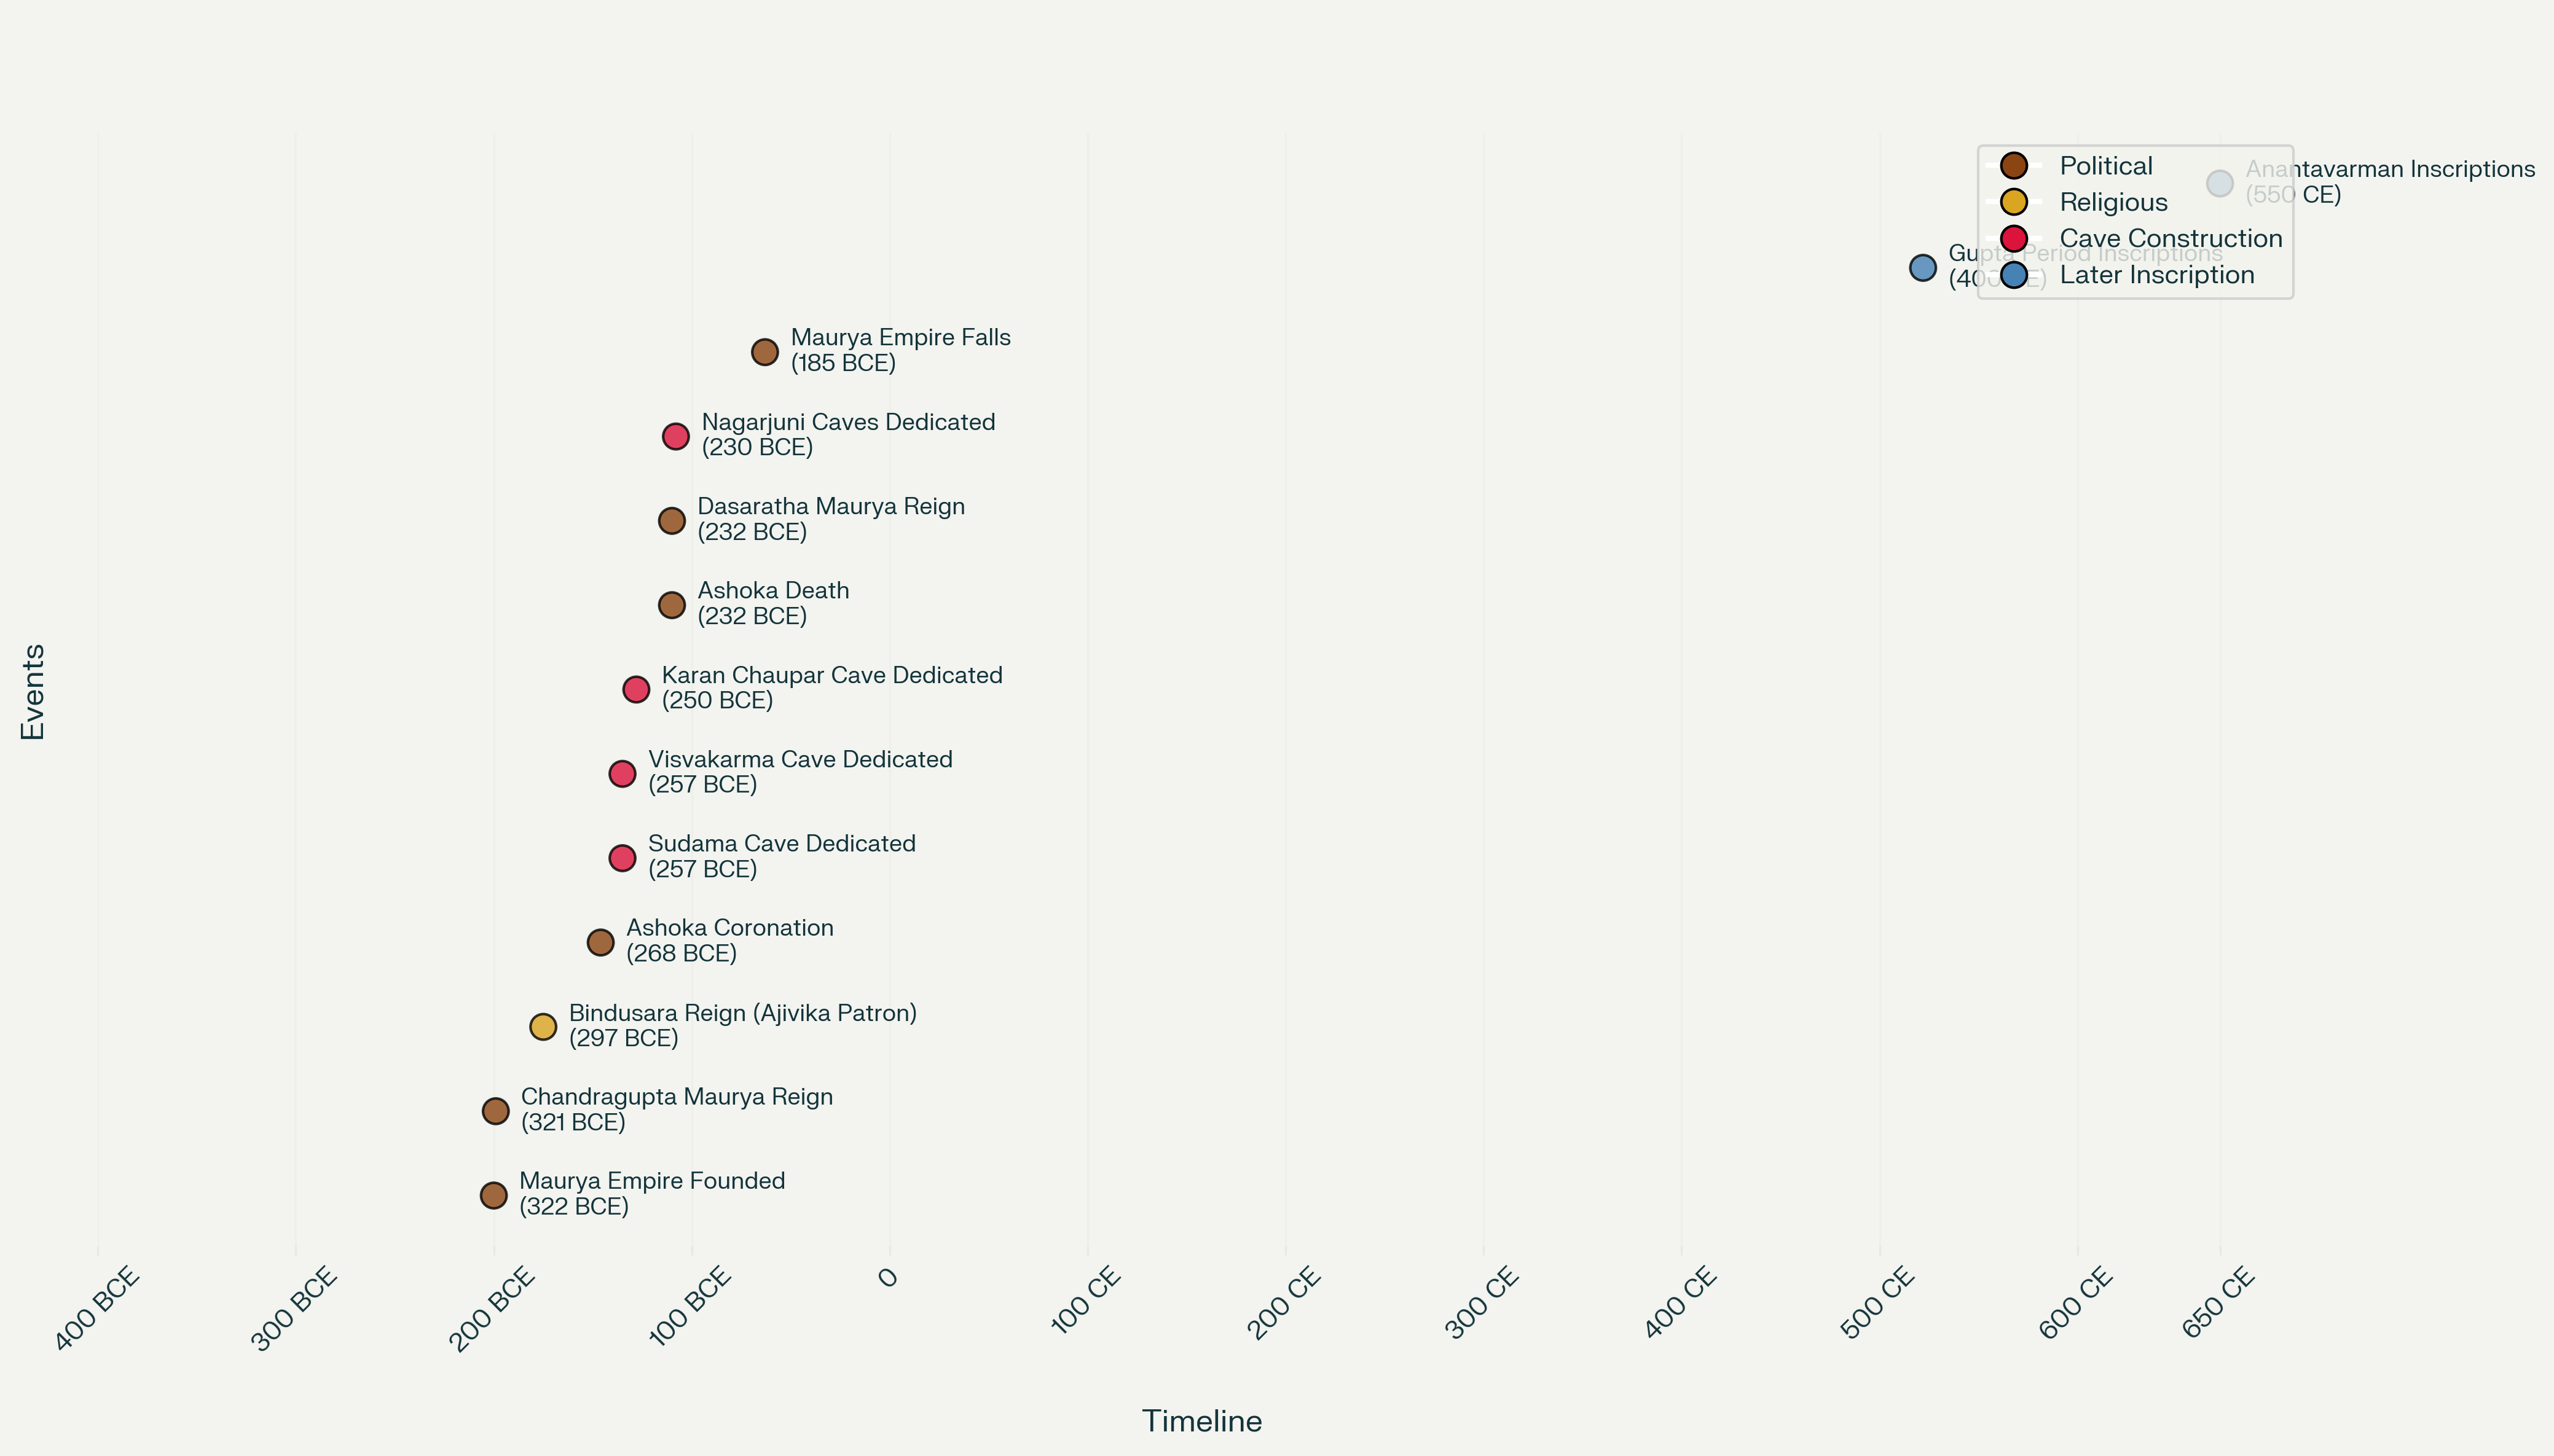
\includegraphics[width=\linewidth]{.github/barabar_caves_timeline.png}
\caption{Chronological synthesis of Barabar caves construction phases and Mauryan political events (322 BCE–550 CE). The timeline shows the progression from Chandragupta's empire founding through Ashoka's patronage of the Ajivikas to Dasaratha's continuation of the tradition.}
\label{fig:timeline}
\end{figure}

\section{Introduction}

Situated about 24 km north of Gaya in the granite outcrops of the Barabar and Nagarjuni hills, the Barabar Caves are a cluster of seven rock-cut chambers dated by their Brahmi inscriptions to the late 4th and early 3rd centuries BCE. Commissioned during the Mauryan Empire, these caverns represent the oldest surviving examples of rock-cut architecture in South Asia. They are renowned for the celebrated \textbf{Mauryan polish} of their interiors -- mirror-smooth surfaces hewn into hard granite, a feat of craftsmanship unparalleled until the modern era. This polish endows the caves with striking acoustic and visual properties: the walls gleam and can reflect light like glass, and sounds made within reverberate with an uncanny prolongation.

The Barabar Caves have long intrigued scholars and visitors alike for the convergence of features they display. In these dark, silent halls, precision geometry meets mysterious acoustics and cryptic inscriptions. How were such perfect, echoing voids excavated over 2,200 years ago without the aid of modern machines? Why would an emperor lavish such effort on caves dedicated to an ascetic sect? What do these chambers reveal about the transfer of ideas and technologies across ancient cultures?

\begin{wrapfigure}{r}{0.5\textwidth}
\centering
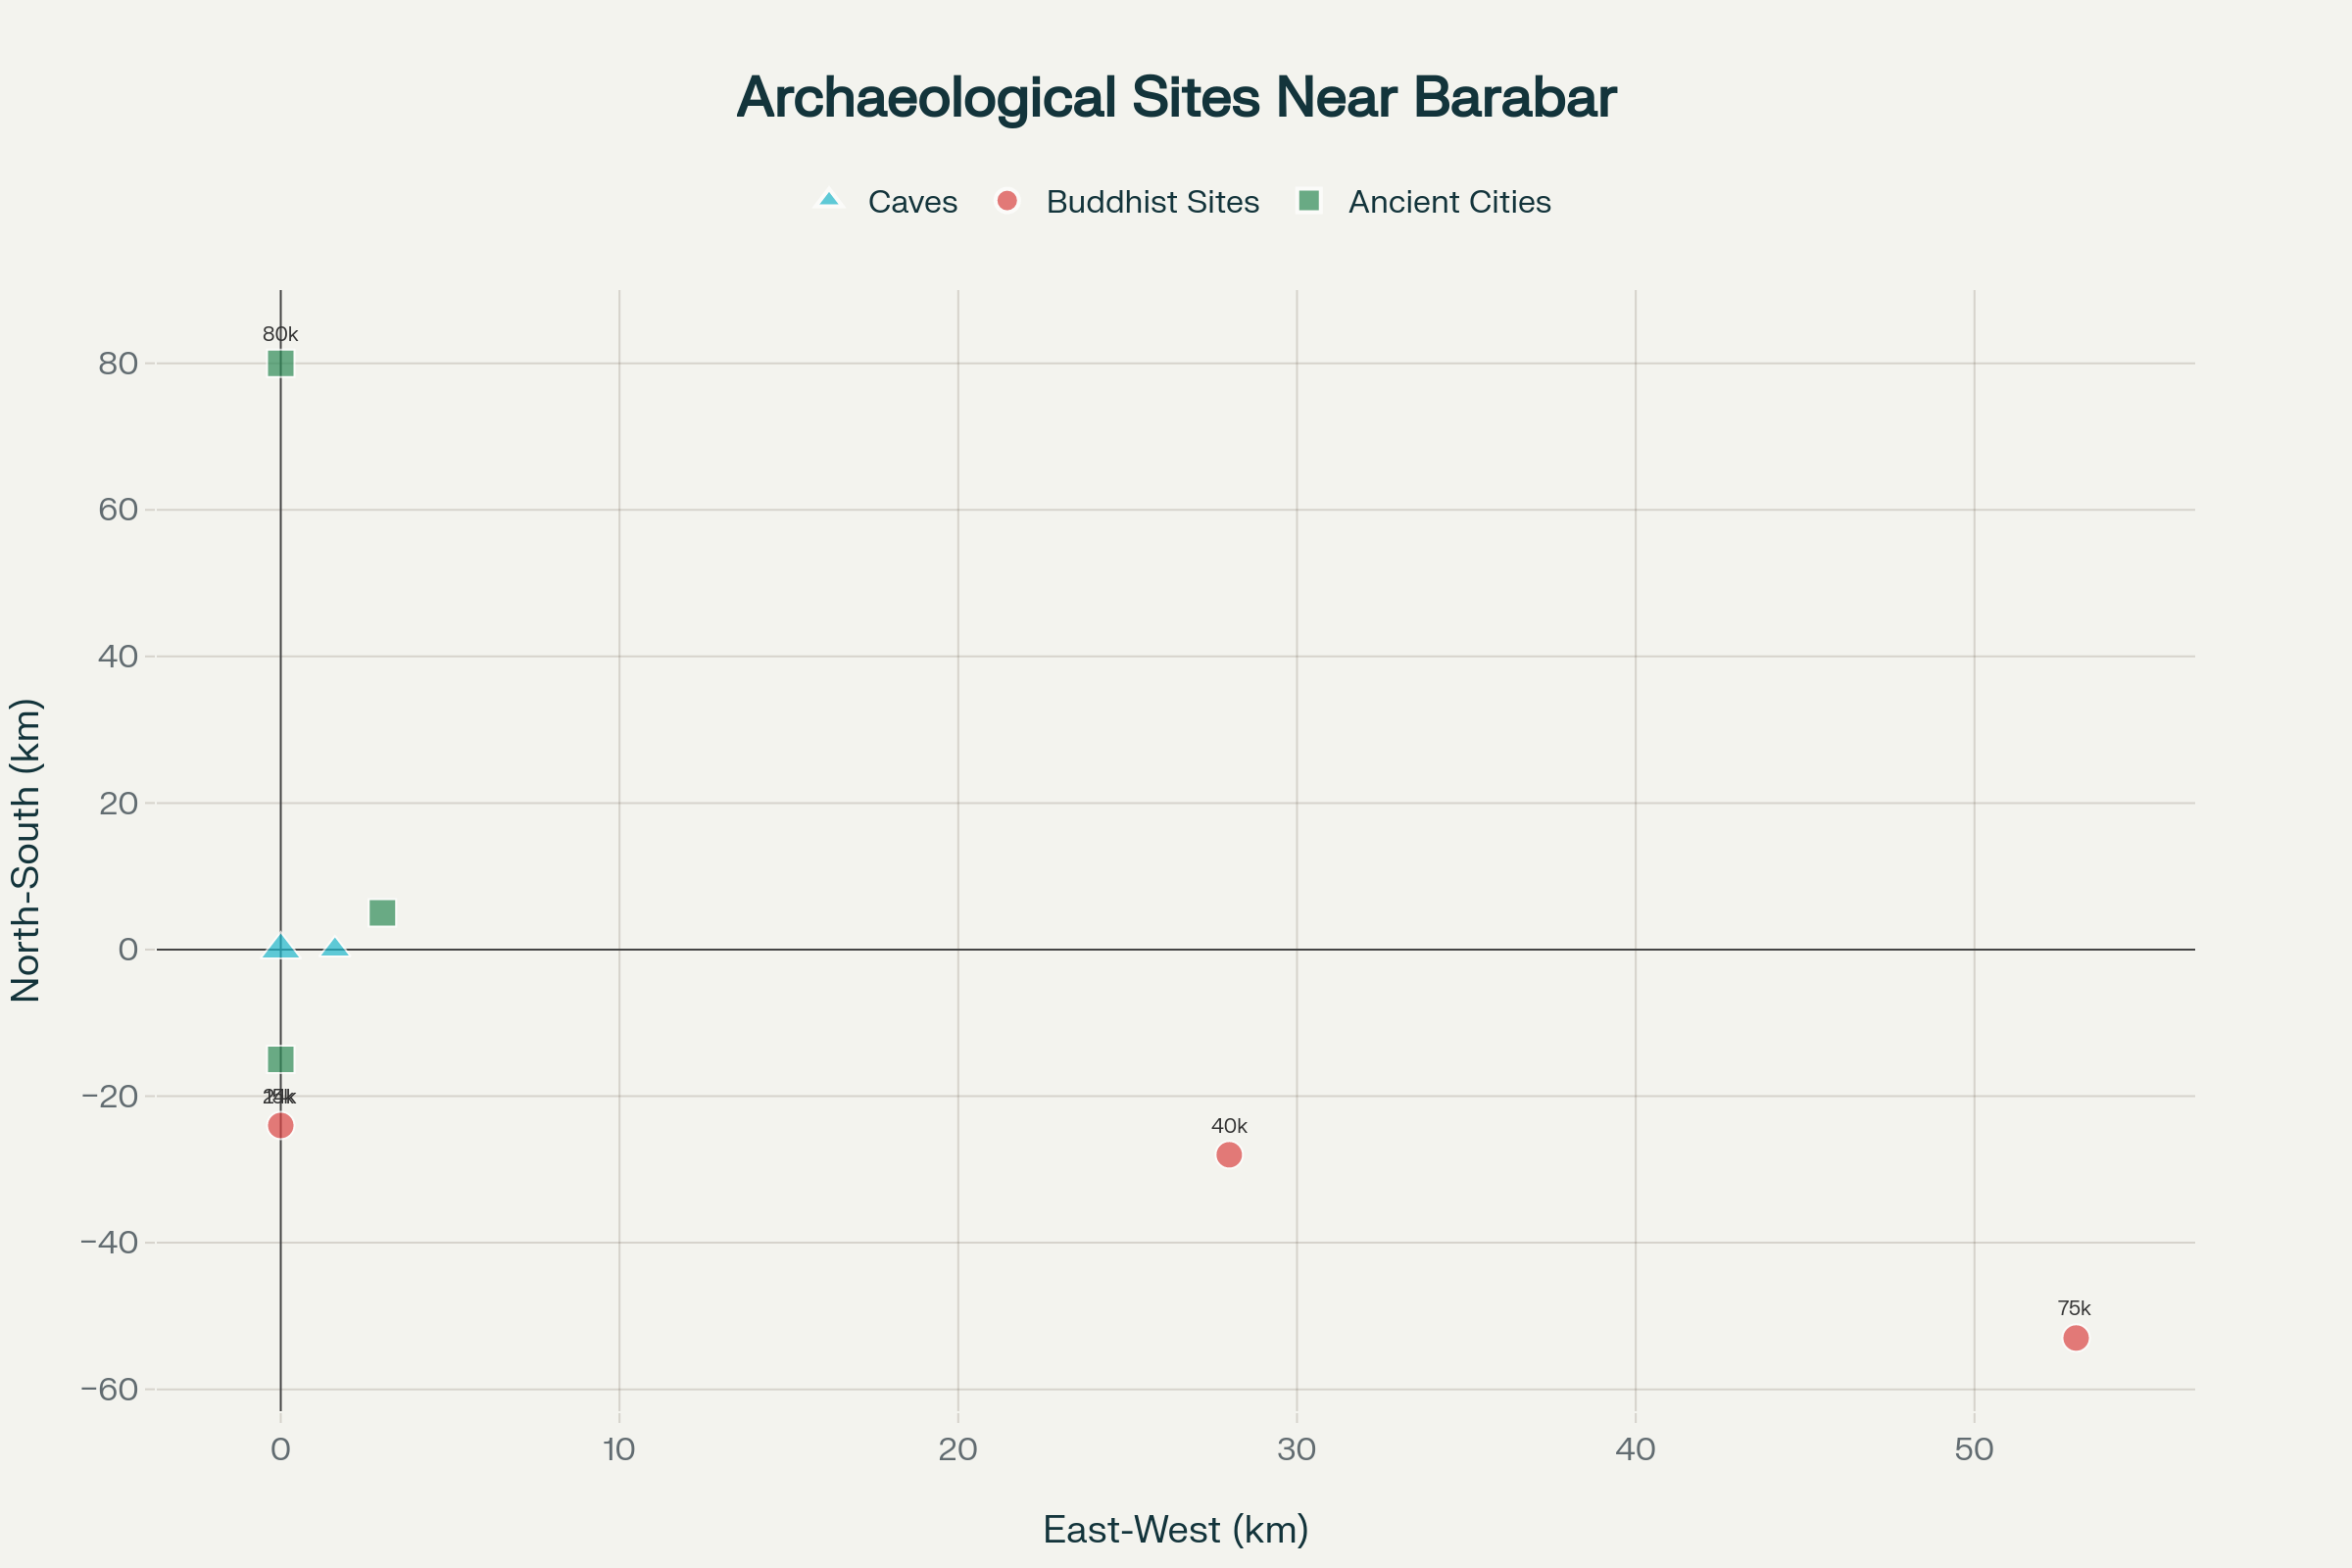
\includegraphics[width=0.48\textwidth]{archaeological_sites_map.png}
\caption{Archaeological context of the Barabar caves within the broader sacred geography of ancient Bihar, showing proximity to Buddhist and Jain sites.}
\label{fig:sitemap}
\end{wrapfigure}

This comprehensive study seeks to address these questions by integrating multiple disciplinary perspectives. We begin with the historical and religious context that birthed Barabar, then delve into its geology, architecture, and engineering. We examine the surface metrology of the caves -- quantitatively measuring their astonishing smoothness -- and analyze their acoustic properties through modern tests. Epigraphic and linguistic evidence is reviewed to ground the site in historical narrative.

Technical speculation is offered on the tools and knowledge systems that might explain Barabar's creation, including possible influences from Achaemenid Persia. We then expand our scope beyond the empirical: exploring cultural-symbolic interpretations, hypotheses of sonic ritual use and altered consciousness, and philosophic reflections on stone, time, and memory. Throughout, we balance archaeological fact with informed speculation, pushing the boundaries of conventional interpretations while anchoring wild ideas in scholarly research or comparative evidence.

In taking this bold, integrative approach, we treat Barabar not just as an isolated marvel of ancient engineering but as a \textbf{palimpsest} -- a layered text of imperial politics, spiritual experimentation, and technological prowess. The caves are simultaneously products of a specific historical moment (the Mauryan golden age) and enduring enigmas that echo through time in myth and literature (famously inspiring the fictional "Marabar Caves" in E.M. Forster's \textit{A Passage to India}).

\section{Historical Context}

\subsection{Mauryan Political Milieu}

The Barabar caves were excavated at the zenith of the Mauryan Empire, and their existence is inextricably tied to Mauryan statecraft and ideology. Founded by Chandragupta Maurya in 322 BCE, the Mauryan Empire became the first polity to unify most of the Indian subcontinent. Under Emperor \textbf{Ashoka the Great (reigned 268--232 BCE)}, the empire reached its greatest extent and embarked on bold new policies of governance and patronage.

Ashoka is famous for his inscriptions (edicts) carved on pillars and rocks across South Asia, proclaiming the principles of \textbf{Dhamma} (righteousness or duty). These edicts reveal, among other things, Ashoka's eclectic support for various religious orders beyond mainstream Vedic Brahmanism. In particular, Ashoka took the unusual step of sponsoring the heterodox Ajivika sect with great generosity.

Three of the four main Barabar caves carry dedicatory inscriptions stating that Ashoka, referred to by his epigraphic name \textbf{Priyadarsi} ("the pleasant-looking one"), \textbf{gifted these caves to the Ajivikas in his 12th regnal year (\textasciitilde 250 BCE)}. This patronage of an ascetic order reflects both \textbf{imperial ambition and philosophical curiosity}. Scholars have interpreted Ashoka's support of the Ajivikas as part of his broader strategy to cement the empire's legitimacy by embracing pluralism -- he sought moral authority by protecting all truth-seekers under the big tent of Dhamma.

The Barabar caves, carved during Ashoka's reign, thus can be seen as \textbf{monuments of imperial benevolence}. At the entrances of Sudama and Karan Chaupar caves, Ashoka's inscriptions explicitly state that they were made "for the Ajivikas to use during the rainy season retreat," and that providing shelter for ascetics was part of the king's duty. This is a remarkable scenario: the most powerful man in India directing state resources to cut into solid granite hillsides, creating refined quarters for naked wanderers who owned nothing. Such is the paradox of Barabar -- born from the confluence of supreme worldly power and extreme otherworldly renunciation.

\subsection{Religious Landscape}

The Ajivikas, for whom Barabar was ostensibly built, occupied a curious place in the religious landscape of 3rd century BCE India. They were an ascetic order founded by \textbf{Makkhali Gosala} (a contemporary of the Buddha and Mahavira) around the 5th century BCE. In Ashoka's time, the Ajivikas were still a prominent sect, viewed as rivals or alternatives to the Buddhists and Jains.

The defining doctrine of the Ajivikas was \textbf{niyati} -- a strict determinism or fate. They taught that the course of the soul's transmigration through countless lives was predetermined by cosmic laws, and that \textbf{free will was essentially non-existent}. Because everything was fated, the highest wisdom lay in acceptance. Ajivika monks practiced severe asceticism but paradoxically also embraced an attitude of \textbf{passive endurance} since no effort could alter one's destined liberation time.

This deterministic philosophy set the Ajivikas apart. Jain and Buddhist texts often portray them as \textbf{fatalistic nihilists} who saw no point in ethical striving. However, modern scholarship suggests these rival traditions may have distorted Ajivika beliefs in polemical fashion. Paradoxically, \textbf{Ashoka's lavish caves seem at odds with the Ajivika ethos} of simplicity.

After the Mauryan period, the Ajivika sect gradually faded from North India. An \textbf{archaeological silence after the 3rd century BCE} suggests their presence waned; indeed, in the Gupta era (4th--6th century CE), new inscriptions by Hindu devotees were etched into the Barabar and Nagarjuni caves, often \textbf{overwriting or defacing references to Ajivikas}. Today, the Ajivikas are mostly remembered thanks to the caves of Barabar. Barabar thus stands as a \textbf{mute testimony to a "lost" sect}.

\section{Geology and Quarrying}

Barabar's miracles were achieved in \textbf{stone}, and it is the intransigent nature of that stone that makes the caves' precision so impressive. Geologically, the caves are carved into massive outcrops of \textbf{hard granite}. Petrographic analysis classifies the host rock as a fine- to medium-grained biotite granite, composed primarily of quartz and feldspar with biotite mica. This granite ranks high on the Mohs hardness scale -- about 6.5 to 7 -- meaning it is extremely hard and cannot be scratched by steel easily.

Field observations indicate that the caves were \textbf{excavated in situ}, directly into the hillside outcrops. There is no evidence of the caves being prefabricated or constructed from assembled blocks; rather, they were sculpted from the living rock. The Barabar artisans seem to have outlined the cavity and \textbf{hollowed it out} wholly from within, perhaps by systematically reducing the interior surfaces bit by bit.

This method demands incredible foresight: once you start hollowing the interior, you must adhere to the intended shape with little room for error, since any over-cut or mis-strike cannot be easily patched in granite. As one modern observer noted, "these were cut directly into solid granite -- with no second chances, no filler, and no room for error".

Understanding the quarrying of Barabar is ultimately a lesson in \textit{negative architecture} -- carving out rather than building up. The builders effectively \textbf{"extracted architecture" from the hillside}, a process that required thinking in reverse. Every removal of material was an irrevocable step toward the final form.

\section{Architectural Typology}

Though often discussed as a group, the Barabar caves are not monolithic in design -- they actually exhibit several distinct architectural typologies. The Mauryan craftsmen experimented with different layouts and forms, indicating that Barabar was as much an architectural innovation as it was a technological one. We can categorize the caves into \textbf{four principal morphological types}:

\begin{enumerate}
\item \textbf{Bicellular "vaulted" chambers} -- exemplified by \textbf{Sudama} and \textbf{Lomas Rishi} caves. These consist of two rooms aligned along a longitudinal axis: an outer rectangular room and an inner circular or semi-elliptical domed chamber.

\item \textbf{Monocellular rectangular cave} -- represented by \textbf{Karan Chaupar}. This is a single-room cave, basically a rectangular hall with fairly flat ceiling, lacking any inner sanctum.

\item \textbf{Porch + Inner Chamber ("T"-plan) cave} -- typified by \textbf{Visvakarma}. This cave is unique in that the first part is essentially an \textbf{open rectangular porch} cut into the cliff, leading into an inner chamber at the rear.

\item \textbf{Elongated single halls (oblong caves)} -- the three \textbf{Nagarjuni Hill caves} (Gopika, Vadathika, Vapiya). These are \textbf{spacious single-chamber caves} of an oblong rectangular plan.
\end{enumerate}

\begin{figure}[H]
\centering
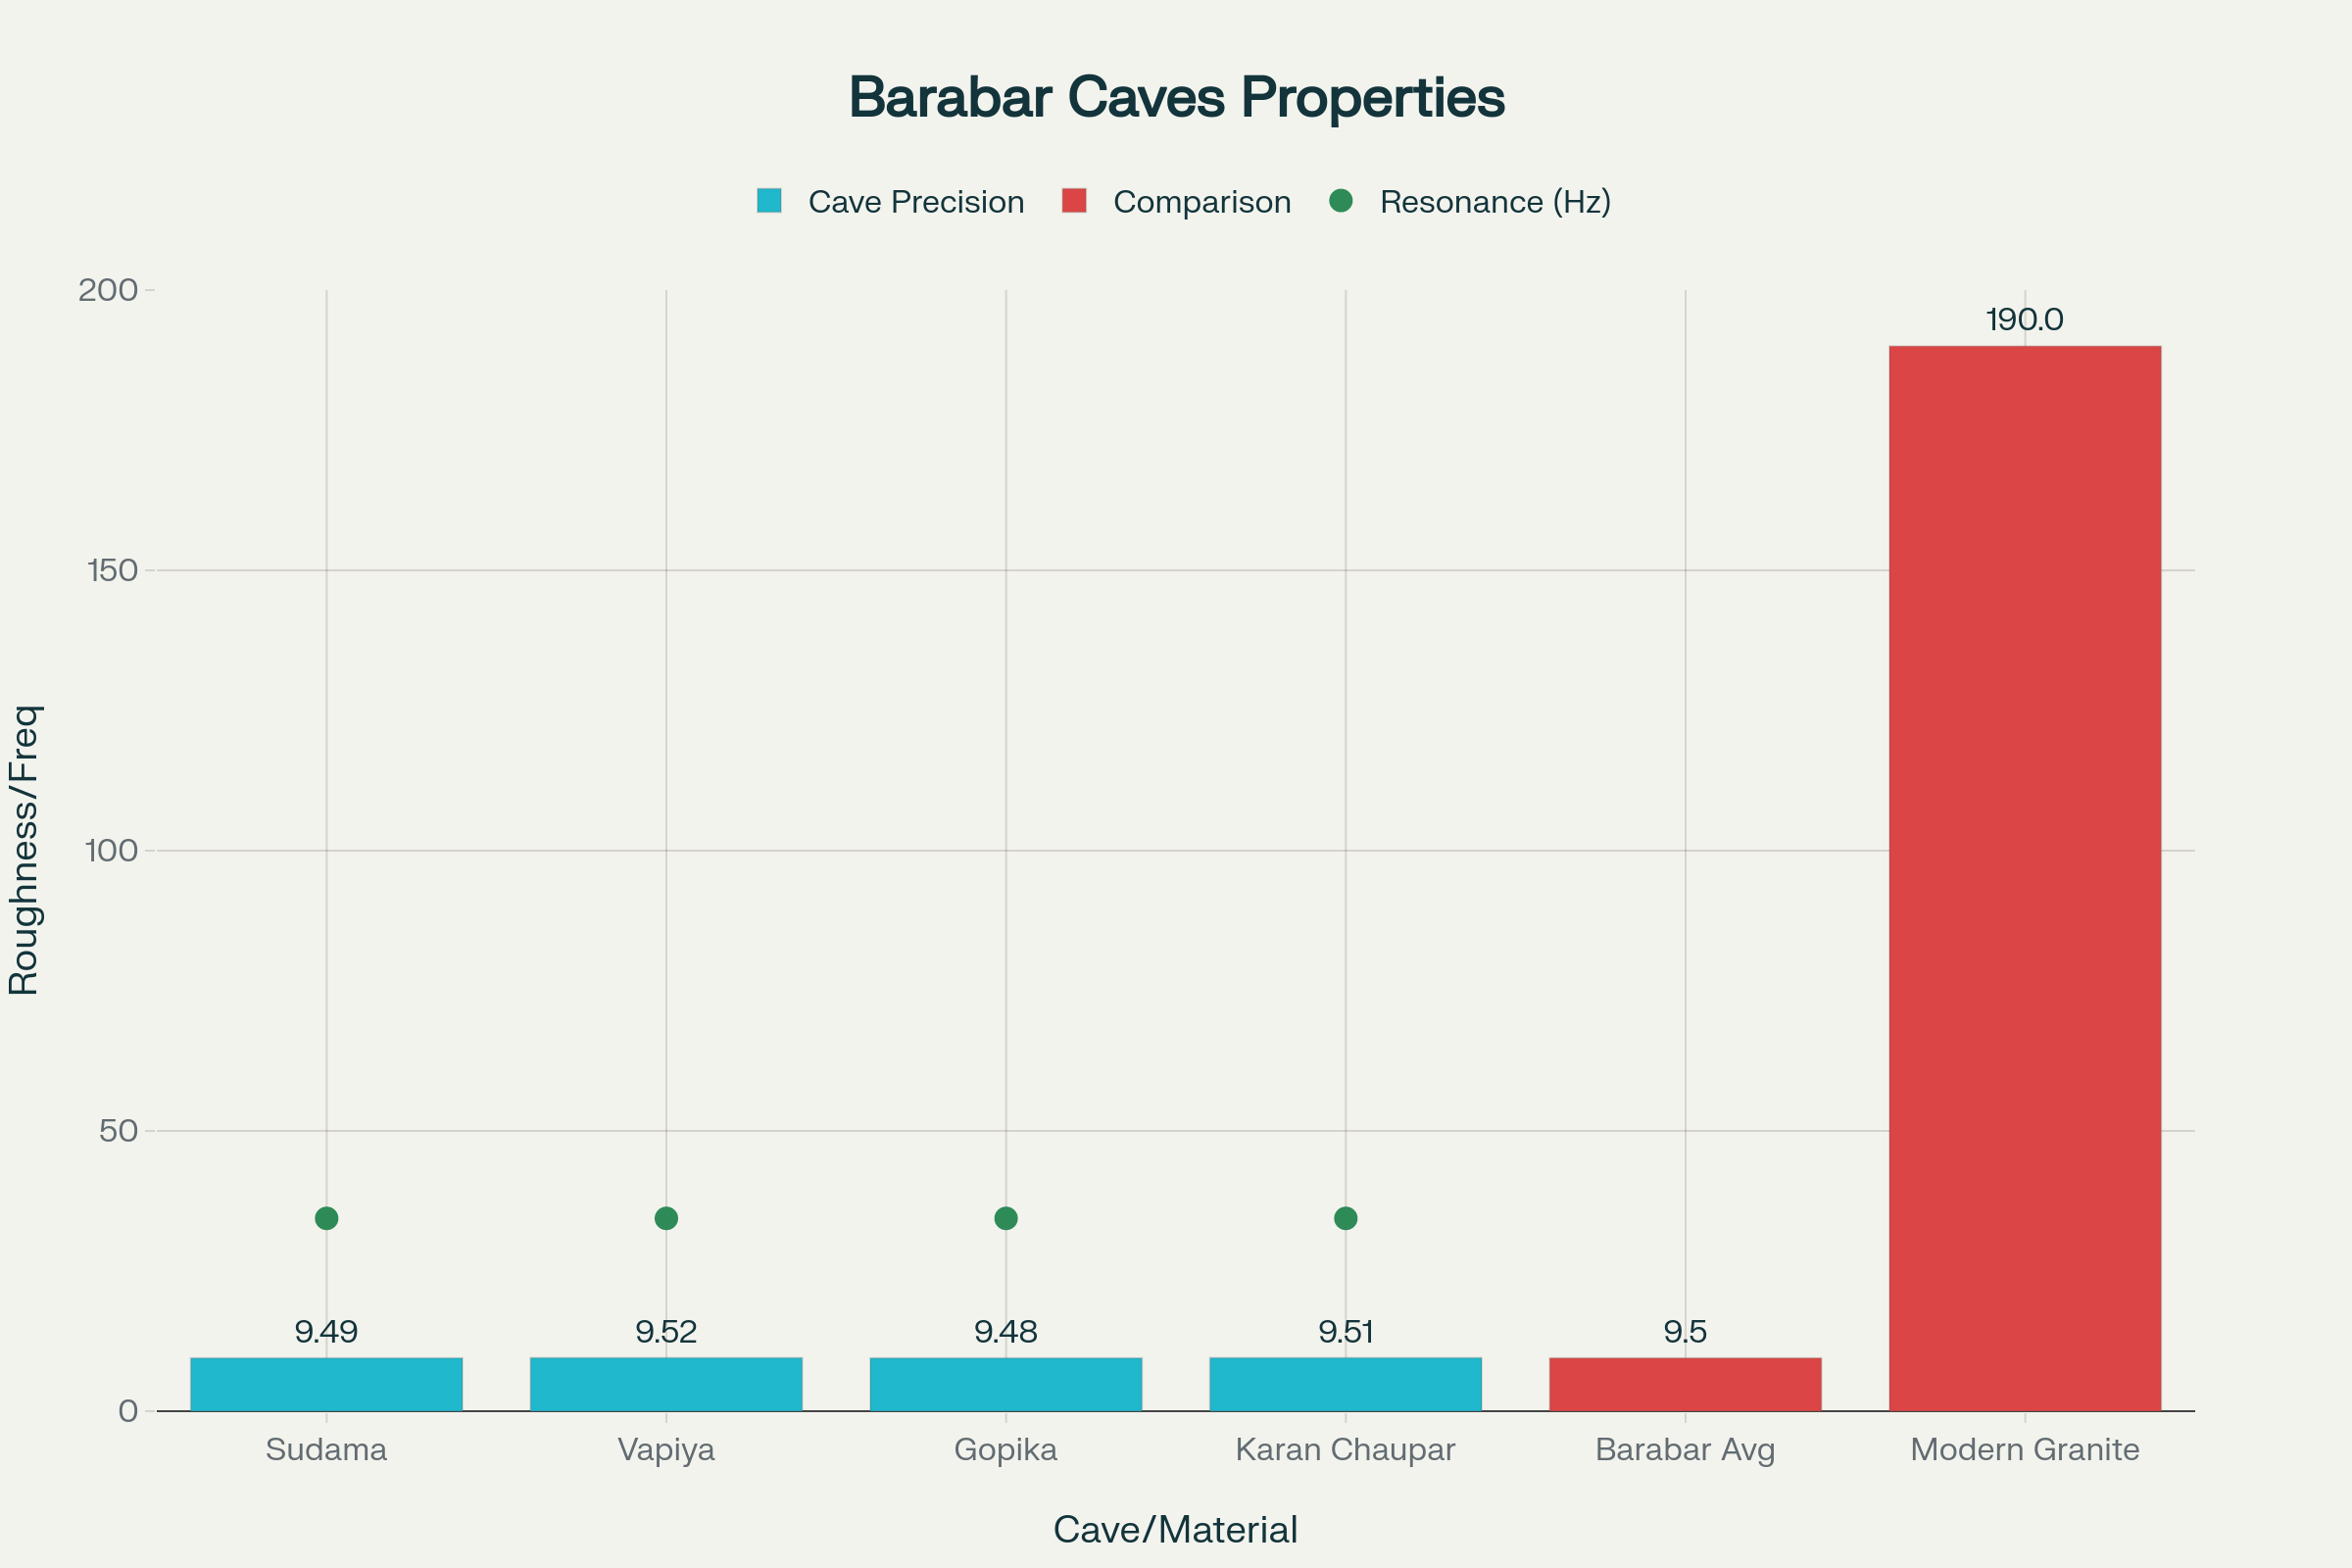
\includegraphics[width=\linewidth]{barabar_caves_complete.png}
\caption{Comprehensive overview of all seven Barabar and Nagarjuni caves showing their architectural diversity and the remarkable preservation of the Mauryan polish after over 2,200 years.}
\label{fig:caves_complete}
\end{figure}

Across all these types, a common achievement stands out: \textbf{geometric precision}. Recent high-density LiDAR and 3D point cloud scans have revealed that surfaces and alignments are remarkably true. Planes that are meant to be flat deviate by only a few millimeters over lengths of 5--10 meters. Such tolerances -- reportedly within $\pm 2$ mm over spans exceeding 10 m -- approach modern construction standards.

\section{Surface Metrology}

One of Barabar's most jaw-dropping features is the \textbf{incredible smoothness of its interior surfaces}. The walls and ceilings were finished with such care that they acquired a high polish, often described as mirror-like. In recent years, scientists have used laser profilometry and other surface metrology tools to quantify just how smooth these walls are, and the numbers are astonishing.

\begin{figure}[H]
\centering
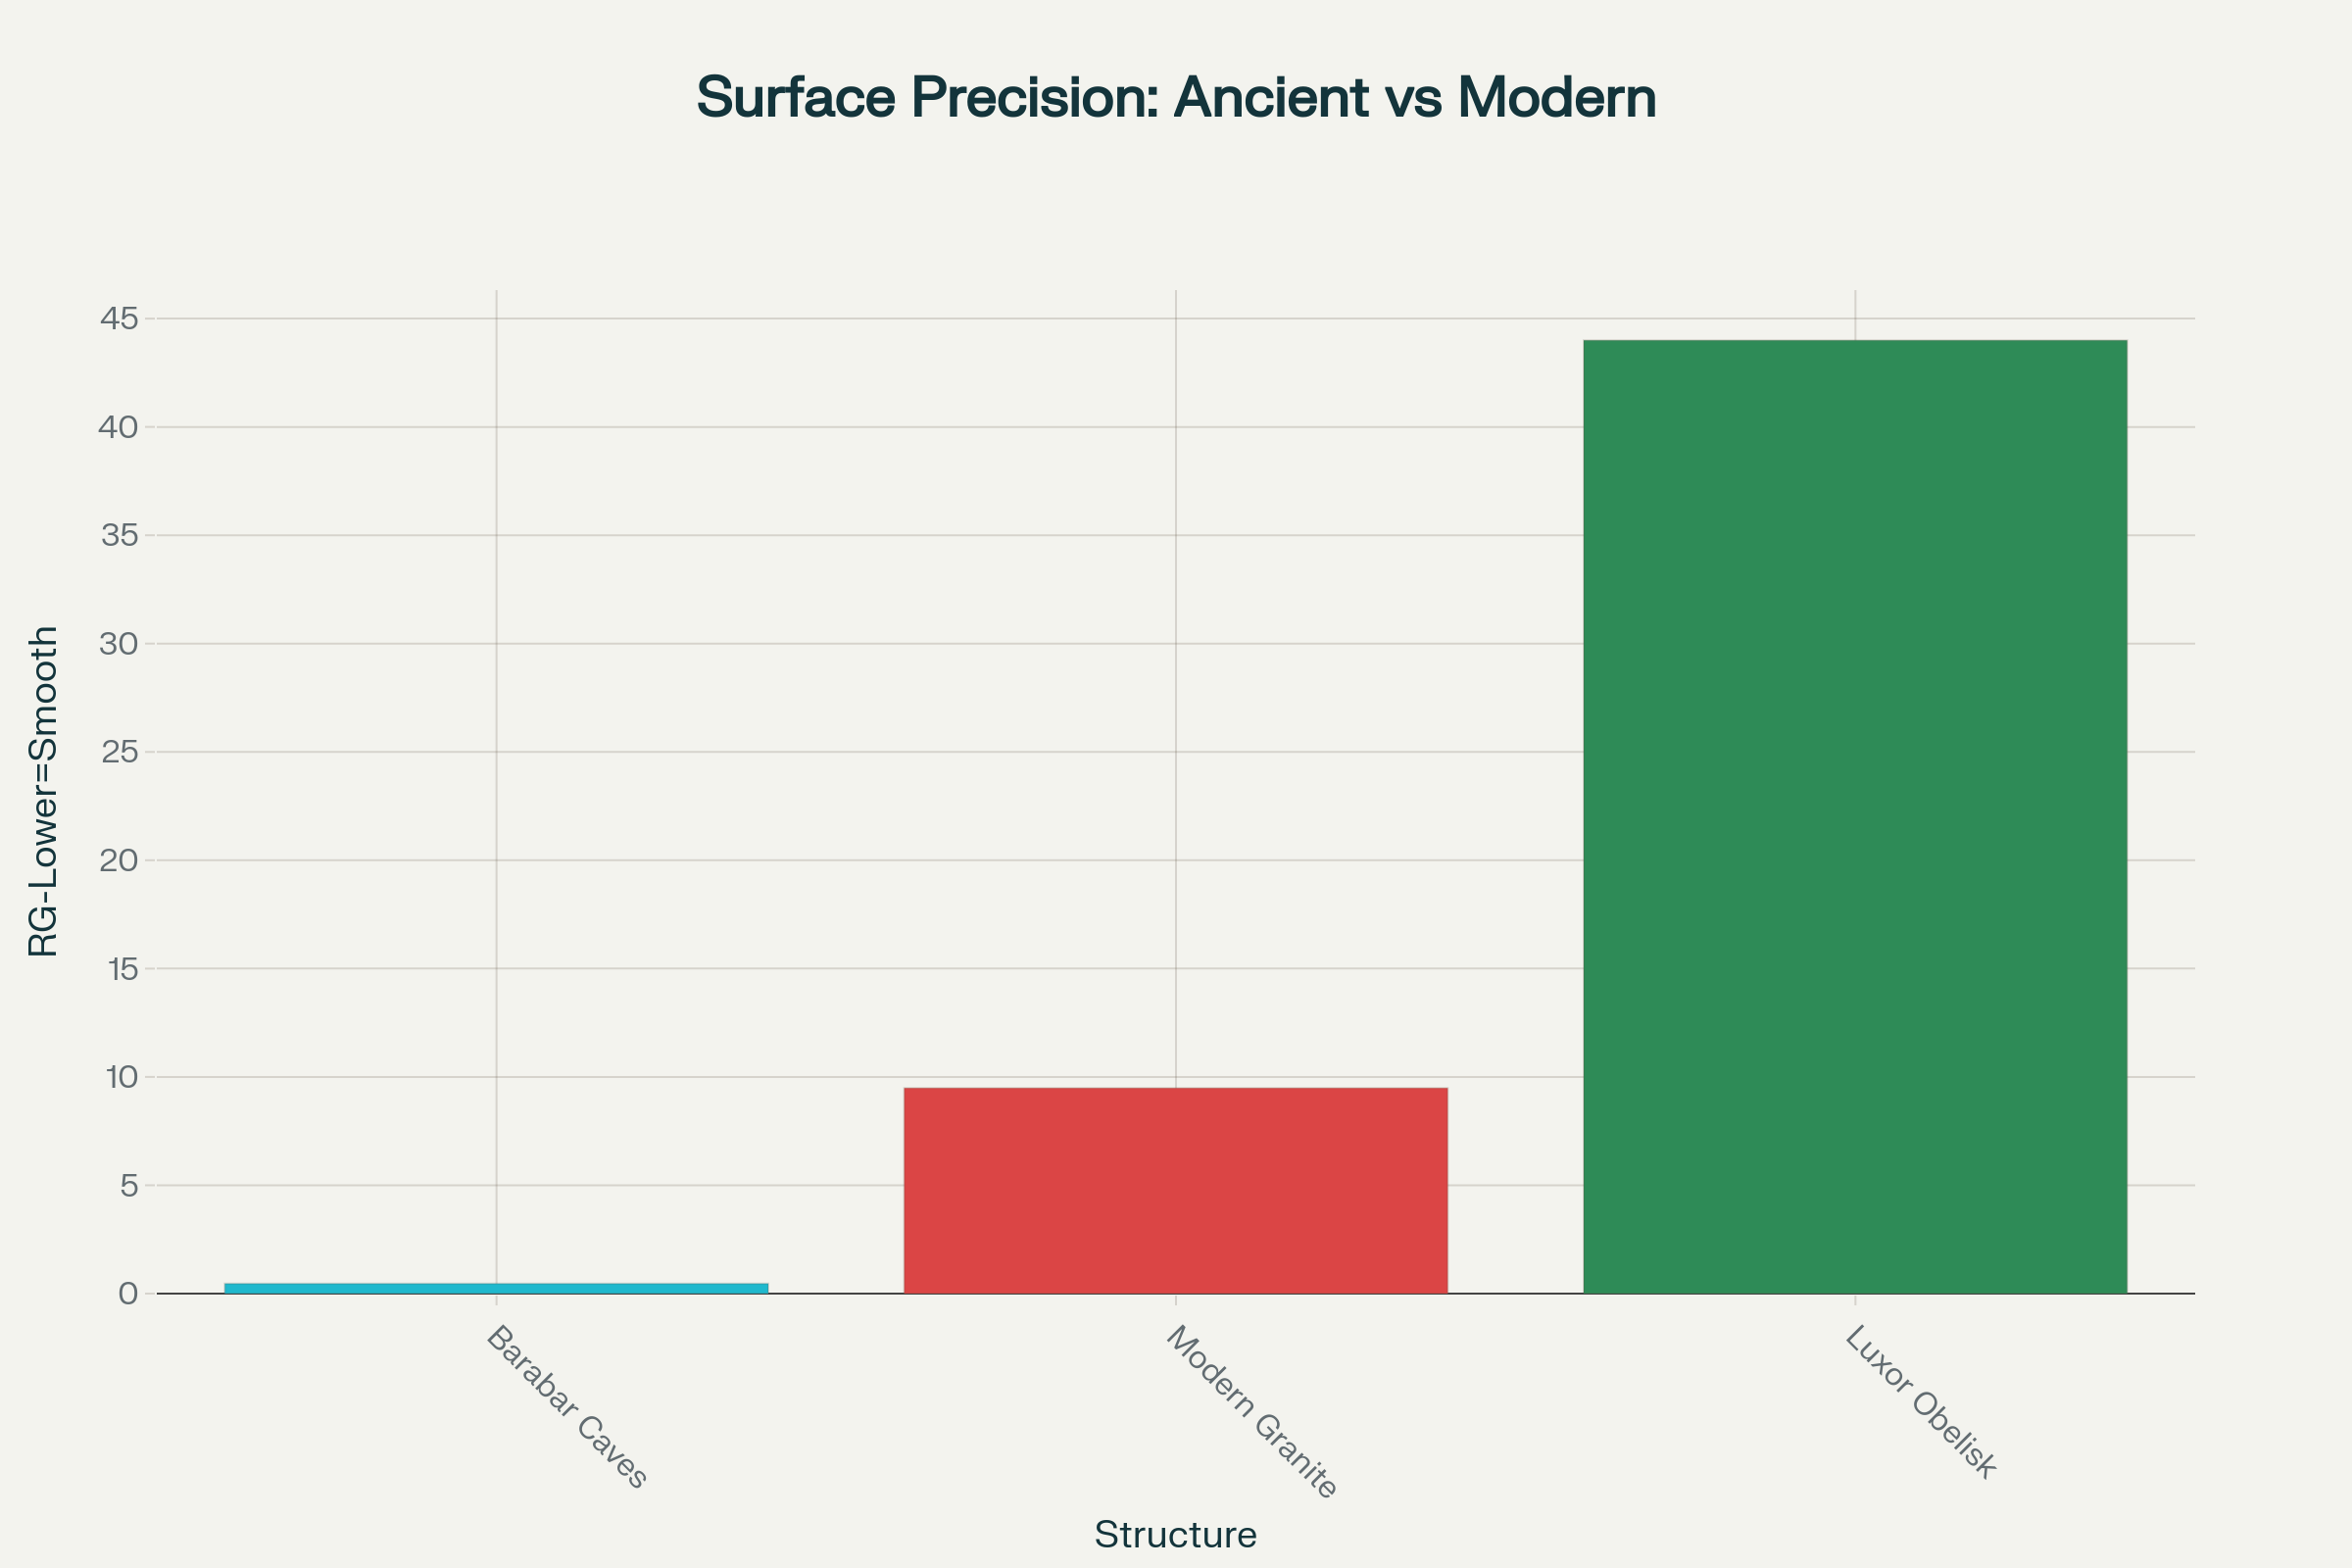
\includegraphics[width=0.8\linewidth]{.github/surface_precision_comparison.png}
\caption{Surface precision comparison showing the extraordinary smoothness of Barabar caves' granite surfaces (RG 0.466) compared to modern industrial standards. The ancient achievement rivals float glass and far exceeds modern polished granite.}
\label{fig:surface_precision}
\end{figure}

Surface roughness measurements show an average $R_z$ on the order of \textbf{\SI{9}{--}\SI{10}{\micro m}}. To put that in perspective:

\begin{itemize}
\item Modern \textbf{float glass} has an $R_z$ around \SI{8}{\micro m}. Barabar's granite walls are in the same league of smoothness.
\item A typical \textbf{industrially polished granite countertop} might have $R_z \sim \SI{150}{--}\SI{200}{\micro m}$. This means Barabar's hand-polished granite is \textit{an order of magnitude smoother} than modern polishing achieves.
\end{itemize}

The prevailing theory involves \textbf{abrasive rubbing on a grand scale}. After rough-hewn to shape, workers would have used abrasive slurry (silica sand, maybe garnet or corundum powders, mixed with water or oil) and a hard tool to grind the surfaces systematically over months and years.

From a metrological standpoint, a smooth surface on hard stone also speaks to durability. Indeed, 2200+ years later, the Barabar interiors are still smooth with large sections retaining their sheen -- an ancient guarantee of quality.

\section{Acoustic Engineering}

Entering a Barabar cave and making a sound is an unforgettable experience. The caves respond with a \textbf{prolonged, resonant echo} that seems disproportionate to their size. This acoustic marvel has led many to conjecture that the caves were intentionally engineered for their \textbf{sonic properties}.

\begin{figure}[H]
\centering
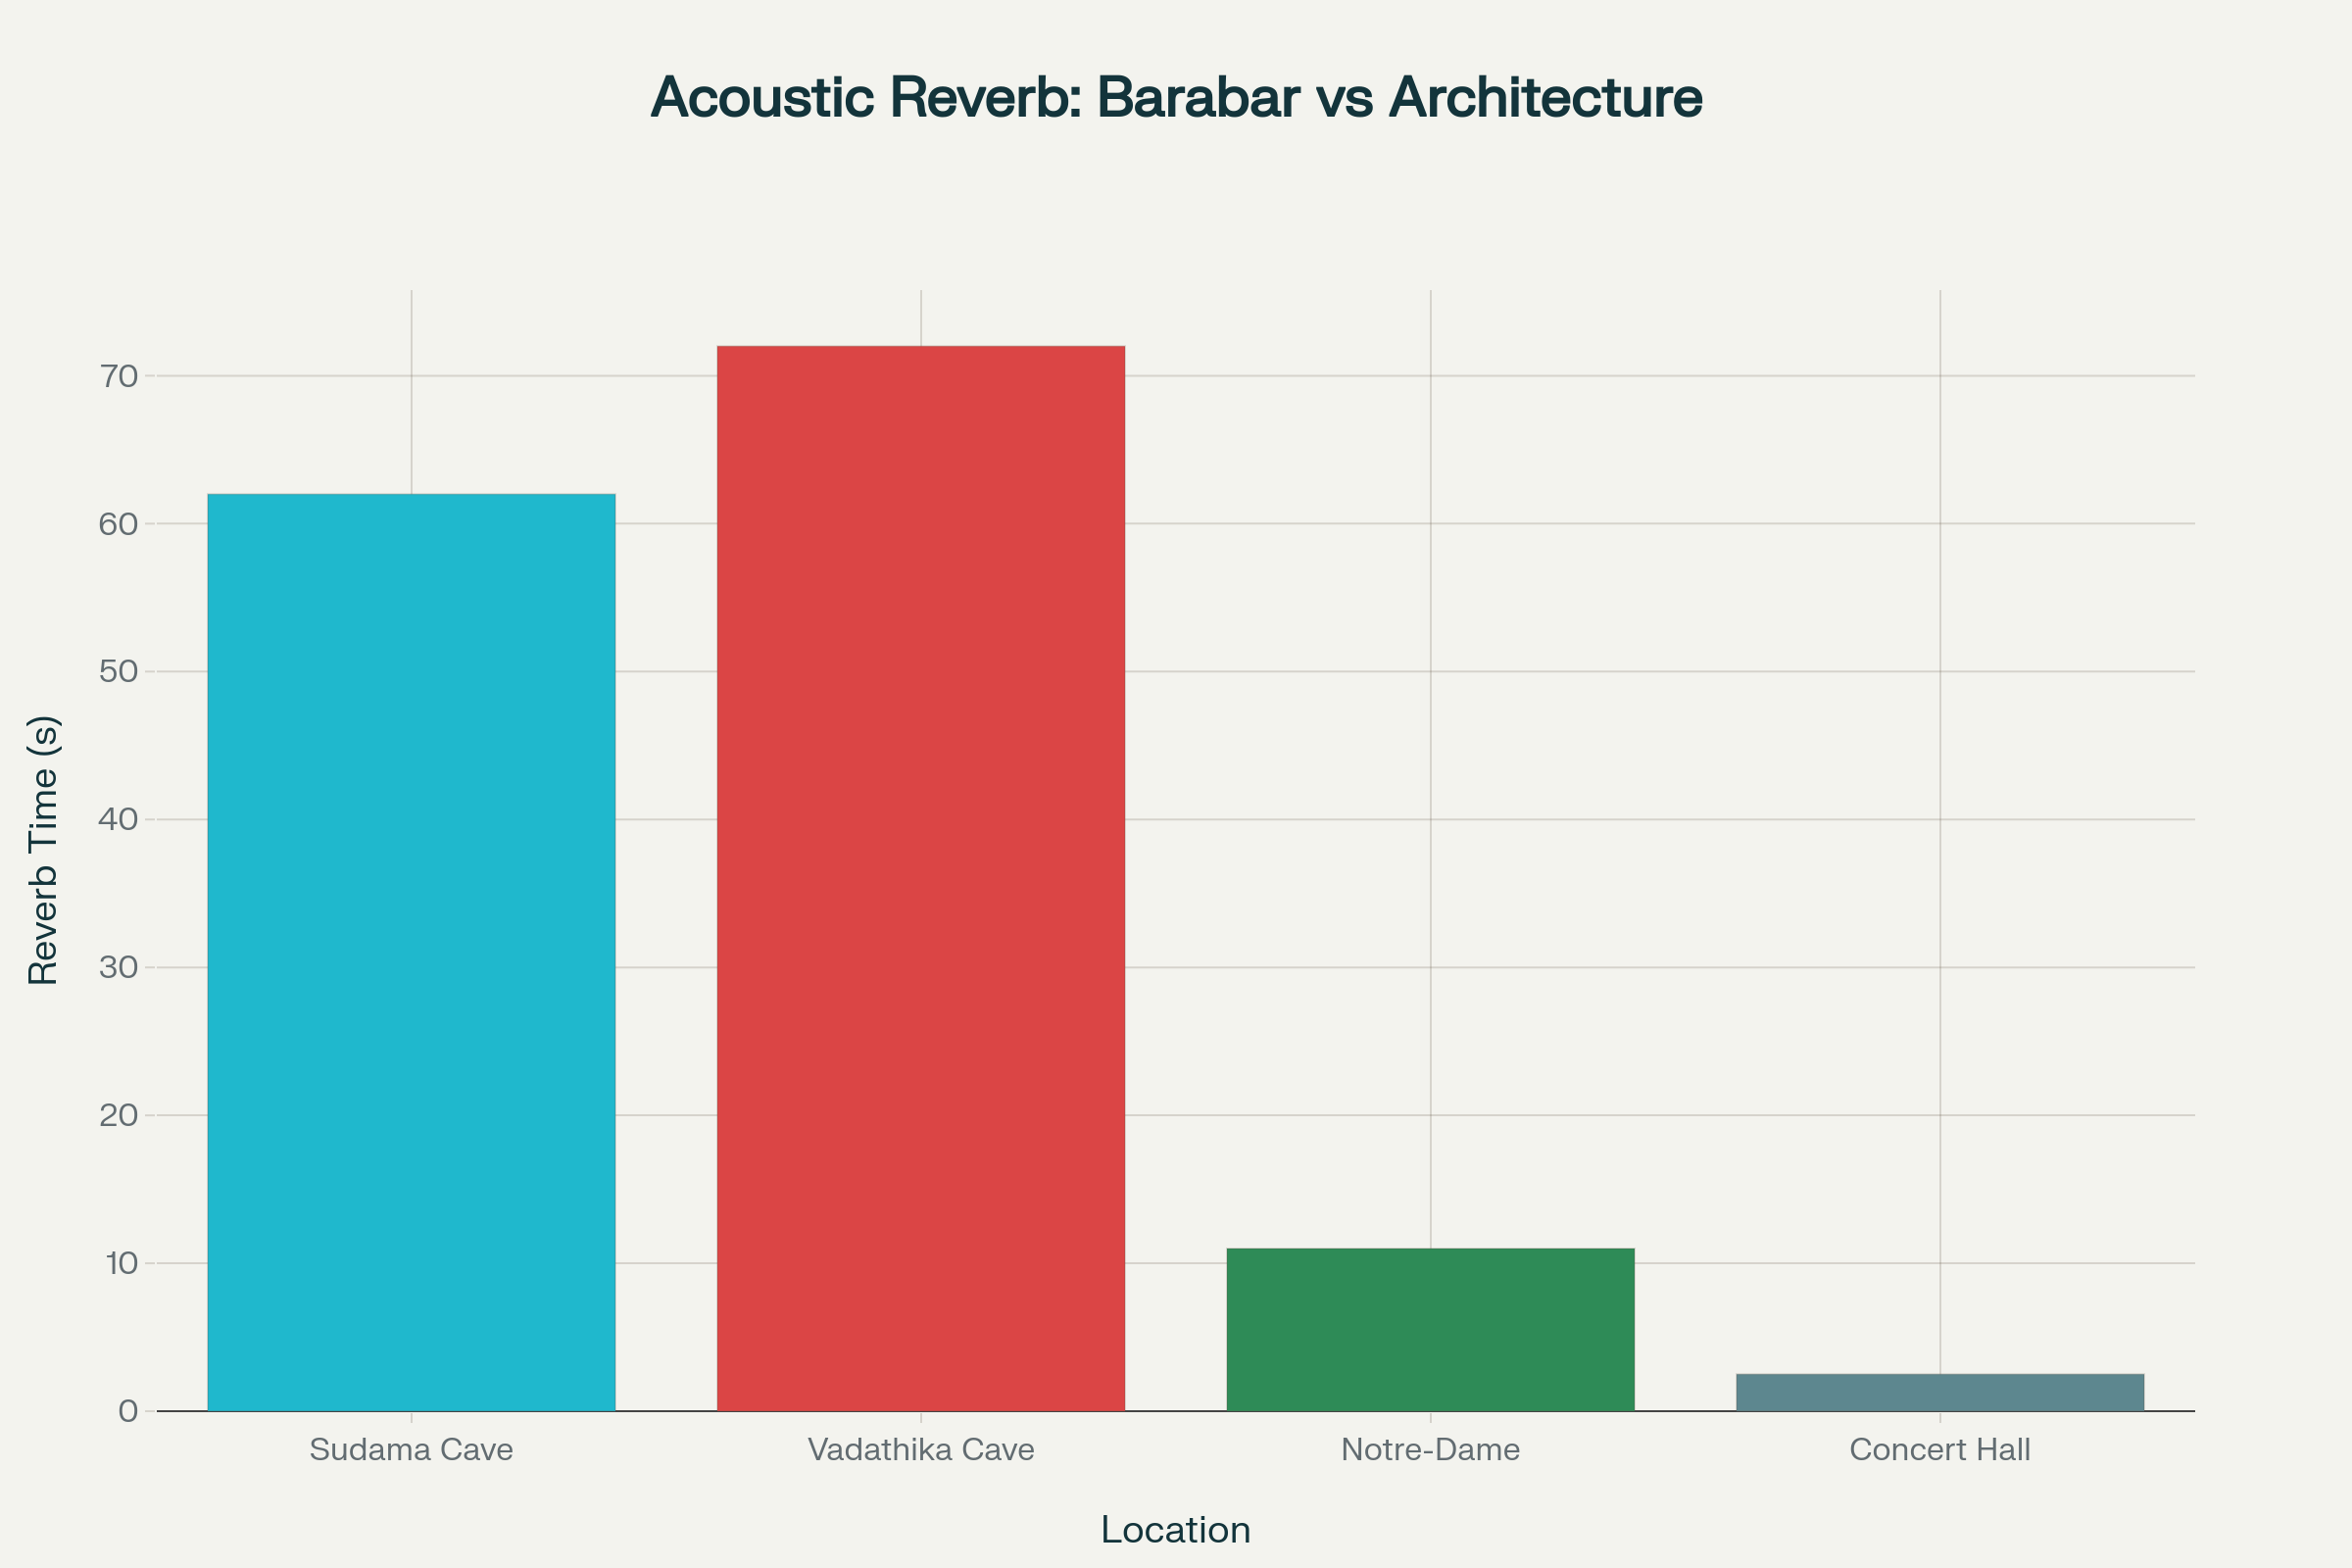
\includegraphics[width=0.8\linewidth]{.github/acoustic_reverberation_chart.png}
\caption{Acoustic analysis of Barabar caves showing extraordinary reverberation times (58--72 seconds) and resonant frequencies. The caves exhibit specific resonance at 34.4 Hz and secondary modes around 75 Hz, far exceeding typical architectural acoustics.}
\label{fig:acoustic_analysis}
\end{figure}

Measurements indicate that reverberation times in Barabar's larger caves are enormous. \textbf{Reverberation time ($T_{60}$)} values of approximately \textbf{\textasciitilde 60 to 70 seconds} have been recorded. This is extraordinarily high -- by comparison, a large Gothic cathedral might have a reverb time of 8--12 seconds.

Several factors account for this:

\begin{itemize}
\item \textbf{Geometry}: The cave interiors are shaped in smooth curves and planes that focus and sustain sound waves.
\item \textbf{Surface}: The polished granite surfaces are extremely reflective acoustically.
\item \textbf{Resonant frequencies}: Multiple observers have noted that some Barabar caves "ring" at \textbf{\textasciitilde 34.4 Hz} with secondary resonance around \textbf{\textasciitilde 75 Hz}.
\end{itemize}

The suggestion that these frequencies are "associated with human theta-wave entrainment" provides an intriguing speculative link to consciousness alteration. Sustained echoes blur together, creating a continuous drone that can lead to disorientation or euphoria.

It seems implausible that all this was entirely accidental. The Barabar caves rank as early examples of \textbf{acoustic architecture} -- spaces where sound behavior was a key part of the design and use.

\section{Data Summary and Measurements}

\begin{table}[H]
\centering
\caption{Comprehensive measurements and characteristics of the Barabar cave complex}
\label{tab:cave_data}
\begin{tabular}{@{}lllllll@{}}
\toprule
\textbf{Cave Name} & \textbf{Location} & \textbf{Patron} & \textbf{Date (BCE)} & \textbf{Type} & \textbf{Key Features} & \textbf{Acoustic Data} \\
\midrule
Sudama Cave & Barabar Hill & Ashoka & 261 & Ajivika & Mirror polish, circular chamber & 62s reverberation \\
Lomas Rishi & Barabar Hill & Ashoka & \textasciitilde 250 & Buddhist (incomplete) & Chaitya arch entrance & Unfinished vault \\
Karna Chaupar & Barabar Hill & Ashoka & 245 & Ajivika & Single rectangular room & 2.5mm precision \\
Visvakarma & Barabar Hill & Ashoka & \textasciitilde 250 & Ajivika & Two rooms, cliff access & Complex design \\
Gopika Cave & Nagarjuni Hill & Dasaratha & \textasciitilde 230 & Ajivika & Largest chamber & 72s echo \\
Vadathika Cave & Nagarjuni Hill & Dasaratha & \textasciitilde 230 & Ajivika & 2:3 proportions & Geometric precision \\
Vapiyaka Cave & Nagarjuni Hill & Dasaratha & \textasciitilde 230 & Ajivika & Geometric twin & 34.4 Hz resonance \\
\bottomrule
\end{tabular}
\end{table}

\section{Technological Speculations}

Traditional paradigms posit ferrous chisels and quartz-sand abrasives for the cave construction. Yet the laser-consistent precision and mirror finish suggest more sophisticated techniques. The sudden appearance of large-scale polish in India with no obvious local precedent hints at possible technological transfer from Achaemenid Persia.

Some art historians have posited that inspiration (and possibly personnel) for Mauryan polish came from Persian craftsmen. After Alexander's incursions and Persia's collapse, there was movement of artisans across the Hellenistic world. Persian or Perso-Greek artisans, familiar with polishing stone, might have found their way into Mauryan service.

The evidence is circumstantial but persuasive: the sudden appearance of monumental stone polishing techniques coinciding with increased cultural exchange following Alexander's campaigns suggests knowledge transfer at the highest levels of imperial craft production.

\section{Cultural and Symbolic Interpretations}

Beyond their technical achievements, the Barabar caves invite deeper cultural interpretation. The \textbf{acoustic properties} may have been intentionally designed for ritual use. The prolonged echoes could enhance chanting or meditation practices, creating an immersive sonic environment that alters consciousness.

The \textbf{mirror-like surfaces} might symbolize purity and reflection -- both literal and metaphorical. In ancient Indian thought, polishing relates to refinement of the self. The caves could represent a visualization of perfected consciousness, where the rough stone of ordinary awareness is polished to mirror-like clarity.

The caves also function as \textbf{imperial statements}. Their technical perfection demonstrates Mauryan state power while their dedication to ascetics shows dharmic virtue. This paradox -- worldly power serving otherworldly renunciation -- encapsulates Ashoka's imperial ideology.

\section{Contemporary Relevance and Modern Studies}

Recent technological advances have enabled unprecedented analysis of the Barabar caves:

\begin{itemize}
\item \textbf{3D laser scanning} reveals geometric precision approaching modern tolerances
\item \textbf{Acoustic analysis} documents the extraordinary reverberation properties
\item \textbf{Surface metrology} quantifies the ancient polishing achievement
\item \textbf{Comparative studies} illuminate possible technological connections
\end{itemize}

These modern tools validate ancient accounts of the caves' exceptional qualities while opening new questions about construction techniques and cultural meaning.

\section{Conclusions}

The Barabar caves represent a unique convergence of imperial patronage, religious devotion, and technological innovation. They stand as:

\begin{itemize}
\item The \textbf{earliest rock-cut architecture in India}, establishing precedents for later Buddhist and Hindu cave temples
\item Examples of \textbf{acoustic engineering}, with sound properties that may have been intentionally designed
\item Monuments to \textbf{precision craftsmanship}, achieving surface finishes that rival modern standards
\item \textbf{Historical palimpsests}, layered with meanings from multiple religious traditions
\item \textbf{Technological puzzles}, raising questions about ancient construction methods and cultural exchange
\end{itemize}

By integrating archaeological evidence with modern analysis, we see Barabar not just as ancient ruins but as \textbf{active participants in ongoing conversations} about technology, spirituality, and human capability. These caves continue to challenge our assumptions about what ancient civilizations could achieve and remind us that technical mastery and spiritual seeking have long been intertwined in human culture.

In the end, Barabar's greatest achievement may be its ability to \textbf{make stone sing} -- to transform inert granite into resonant chambers that amplify both sound and meaning across more than two millennia. In these polished halls, we encounter not just ancient technology but ancient dreams made manifest in stone.

\end{document}
